% --------------------------------------------------------------
% This is all preamble stuff that you don't have to worry about.
% Head down to where it says "Start here"
% --------------------------------------------------------------
 
\documentclass[12pt]{article}
 
\usepackage{subcaption}
\usepackage[margin=1in]{geometry} 
\usepackage{amsmath,amsthm,amssymb,scrextend}
\usepackage{fancyhdr}
\usepackage{enumitem}
\usepackage{amsmath}
\usepackage{amssymb}
\usepackage{textcomp}
\usepackage{fancybox}
\usepackage{tikz}
\usepackage{tasks}
\pagestyle{fancy}
\usepackage[makeroom]{cancel}
\usepackage{graphicx}
\usepackage{caption}
\usepackage{mwe}
\usepackage{tikz}
\usetikzlibrary{positioning}

\newcommand{\N}{\mathbb{N}}
\newcommand{\Z}{\mathbb{Z}}
\newcommand{\I}{\mathbb{I}}
\newcommand{\R}{\mathbb{R}}
\newcommand{\Q}{\mathbb{Q}}
\renewcommand{\qed}{\hfill$\blacksquare$}
\let\newproof\proof
\renewenvironment{proof}{\begin{addmargin}[1em]{0em}\begin{newproof}}{\end{newproof}\end{addmargin}\qed}
% \newcommand{\expl}[1]{\text{\hfill[#1]}$}
 
\newenvironment{theorem}[2][Theorem]{\begin{trivlist}
\item[\hskip \labelsep {\bfseries #1}\hskip \labelsep {\bfseries #2.}]}{\end{trivlist}}
\newenvironment{lemma}[2][Lemma]{\begin{trivlist}
\item[\hskip \labelsep {\bfseries #1}\hskip \labelsep {\bfseries #2.}]}{\end{trivlist}}
\newenvironment{problem}[2][Problem]{\begin{trivlist}
\item[\hskip \labelsep {\bfseries #1}\hskip \labelsep {\bfseries #2.}]}{\end{trivlist}}
\newenvironment{exercise}[2][Exercise]{\begin{trivlist}
\item[\hskip \labelsep {\bfseries #1}\hskip \labelsep {\bfseries #2.}]}{\end{trivlist}}
\newenvironment{reflection}[2][Reflection]{\begin{trivlist}
\item[\hskip \labelsep {\bfseries #1}\hskip \labelsep {\bfseries #2.}]}{\end{trivlist}}
\newenvironment{proposition}[2][Proposition]{\begin{trivlist}
\item[\hskip \labelsep {\bfseries #1}\hskip \labelsep {\bfseries #2.}]}{\end{trivlist}}
\newenvironment{corollary}[2][Corollary]{\begin{trivlist}
\item[\hskip \labelsep {\bfseries #1}\hskip \labelsep {\bfseries #2.}]}{\end{trivlist}}
 
\setlength{\parindent}{0pt}
\begin{document}
 \settasks{
	counter-format=(tsk[r]),
	label-width=4ex
}
\newcommand\independent{\protect\mathpalette{\protect\independenT}{\perp}}
\def\independenT#1#2{\mathrel{\rlap{$#1#2$}\mkern2mu{#1#2}}}
% --------------------------------------------------------------
%                         Start here
% --------------------------------------------------------------

\lhead{Math 632}
\chead{Continuous Time Markov Chains}
\rhead{Meenmo Kang}

Philosophically exactly like in discrete time: given the present state, the past and the future are independent. But the math becomes more technical. Throughout, the state space $S$ is finite or countably infinite.\\

{\bf Definition} Let $\{X_t:0\le t< \infty\}$ be a stochastic process. Then $X$ is a Markov chain if for all $0\le s_0<\ldots<s_n<s<t$ and all $x_0,\ldots,x_n,x,y\in S:$
$$P(X_t=y\;|\;X_s=x,\;X_{s_n}=x_n,\ldots,X_{s_0}=x_0) = P(X_t=y\;|\;X_s=x)$$ 
wherever the conditioning event has positive probability.

\vspace{1\baselineskip}
We will only deal with the time-homogeneous case where
$$P(X_t=y\;|\;X_s=x) = P(X_{t-s}=y\;|\;X_0=x)$$
The \underline{transition probability} is 
$$P_t^{(x,y)} = P(X_t=y\;|\;X_0=x)$$

Since there are \underline{uncountably} many transition matrices $\{P_t(x,y)\}_{x,y\in S},$ the transition probability is not as useful as in discrete time. It even turns out to be extremely had to calculate in some cases.


\begin{figure}[!htbp]
    \centering
    \begin{subfigure}[b]{0.3\textwidth}
        \includegraphics[height=5cm, width=6.5cm]{CTMC_1.jpeg}
        \caption{Discrete-Time MC}
    \end{subfigure}\qquad\qquad
    \begin{subfigure}[b]{0.3\textwidth}
        \includegraphics[height=5cm, width=6.5cm]{CTMC_1.jpeg}
        \caption{Continuous-Time MC}
    \end{subfigure}
\end{figure}

The Markov property \underline{force} the holding times $t_1,t_2,t_3,...$ to be exponential random variables. By the same token, the sequence of states visited has to be a discrete-time Markov chain.

\vspace{1\baselineskip}
{\sl Recall the following:}\\
Let $\eta_1,\eta_2,...,\eta_n$ be independent. $\eta\sim\Exp(\lambda)$. $\zeta = \min\{\eta_1,...,\eta_n\}$. I = the index $i$ s.t. $\eta_1 = \zeta$.
$$\zeta \independent I \qquad \zeta\sim\exp(\lambda_1+\ldots+\lambda_n)$$
$$P(\zeta>t)=\prod\limits_{i=1}^n P(\eta_i > t) = \prod\limits_{i=1}^n e^{-\lambda_i t} = e^{-(\lambda_1+\ldots+\lambda_n)t}\qquad\;\;
P(I=1) = \frac{\lambda_i}{\sum\limits_{j=1}^n \lambda_j}$$

\newpage
{\bf Special case} Let $(Y_n)$ be a discrete-time Markov chain with transition matrix $u=(u(x,y))_{x,y\in S}$. Let $N(t)$ be a rate $\lambda$ Poisson process. Then $X_t = Y_{N(t)}$ is a continuous time Markov chain.

In this {\bf SPECIAL CASE} we can calculate the transition probability:
\begin{align}
    P_t(x,y) &= P(x_t=y\;|\;X_0=x) = P(X_t=y\;|\;Y_0=x) \nonumber \\
    &=\sum\limits_{n=0}^\infty P(X_t=y,\;N(t)=n\;|\;Y_0=x) \nonumber \\
    &\text{\quad (N(t): the number of jumps by time t)} \nonumber \\
    &=\sum\limits_{n=0}^\infty P(Y_n=y,\;N(t)=n\;|\;Y_0=x) \nonumber \\ 
    &=\sum\limits_{n=0}^\infty P(N(t)=n)P(Y_n=y\;|\;Y_0=x) \nonumber \\
    &= \sum\limits_{n=0}^\infty \frac{e^{-\lambda t} (\lambda t)^n}{n!} \cdot u^n(x,y) \nonumber
\end{align}

Note that $Z\sim$ Poisson($\mu$) then
$$P(Z=k) = \frac{e^{-\mu}\mu^k}{k!}$$

\vspace{1\baselineskip}
What takes the place of the transition probabilities as the fundamental object? {\bf Rates}.\\

{\bf Definition} For $x\neq y$ in $S$, the \underline{Rate} of jumping from $x$ to $y$ is 
$$q(x,y)=\lim\limits_{h\to 0} \frac{P_h(x,y)}{h}$$
This limit will exist in all our examples. \\

\vspace{1\baselineskip}
Note that 
$$u^{(0)}(x,y) = \begin{cases} 1&x=y\\0&x\neq y\end{cases}$$
$$u^{(0)} = I = \text{the identity matrix}$$

\vspace{1\baselineskip}
Back to the previous {\bf SPECIAL CASE:}
\begin{align}
    \frac{1}{h}p_h(x,y) &= \frac{1}{h} \sum\limits_{n=0}^\infty \frac{e^{\lambda h}(\lambda h)^n}{n!} u^n(x,y) \nonumber \\
    &\vdots \nonumber \\
    &\text{n=0\; term = 0!} \nonumber \\
    &\vdots \nonumber \\
    &=\underbrace{0}_{n=0} \underbrace{e^{-\lambda h}\lambda u(x,y)}_{\substack{{n=1}\\ \text{$\lambda u(x,y)$ as $h\to 0$}}} + \underbrace{\frac{1}{h} \sum\limits_{n=2}^\infty \frac{\overbrace{e^{-\lambda h}}^{\le 1}(\lambda h)^n}{n!} \overbrace{u^{(n)}(x,y)}^{\le 1}}_{\substack{{0\le \cdot \le \frac{1}{h}h^2\sum\limits_{n=2}^\infty \frac{\lambda^n h^{n-2}}{h!}}\\ {\le h \sum\limits_{n=2}^\infty \frac{\lambda^n}{n!} \le h e^\lambda}
    \\ \text{This term doesn't matter later on}}} \nonumber
\end{align}

\vspace{1\baselineskip}
Hence $$q(x,y)=\lambda u(x,y)$$ where $\lambda$ is the rate of Poisson clock and $u(x,y)$ is the probability of jumping to $y$.

\vspace{1\baselineskip}
"little oh of h" o(h) means a quantity that when divided by $h$ goes to o as $h\to \mathcal{O},\;\frac{\mathcal{O}(h)}{h}\xrightarrow{h\to 0}$

\vspace{1\baselineskip}
\rightarrow \text{Hence forth we will give our examples in terms of rates.}

\vspace{1\baselineskip}
{\sl Ex.} Let $N(\cdot)$ be a rate $\lambda$ Poisson process. Then $N(\cdot)$ is a Markov chain with stable space $S=Z_{\ge 0}$ and rates

\newpage
{\bf Continuous Time Markov chains are determined by the rates}
$$q(x,y) = \lim\limits_{h\to 0} \frac{p_h(x,y)}{h} = \text{exponential rate of jumping to $y$, when the present state is $x$}$$

\vspace{1\baselineskip}
Given rates $\{q(x,y)\}_{x\neq y}$
\begin{enumerate}
    \item Construct the Markov chain $X_t$
    \item Compute transition probability $P_t = (p_t(x,y))_{x,y\in S}$
    \item Determine invariant distributions
\end{enumerate}


\vspace{2\baselineskip}
\begin{enumerate}
    \item  Construct the Markov chain $X_t$. Suppose $X_0=1$.
        \begin{itemize}
        \item $S = \{1,2\}$. \\
        
        $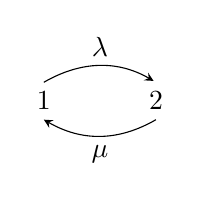
\begin{tikzpicture}
        \node (a) {1};
        \node[right=1cm of a] (b) {2};
        
        %a>b
        \draw[-stealth,shorten >= 1pt] (a.north) to[bend left] node[midway,above] {$\lambda$} (b.north);
        %b>a
        \draw[-stealth] (b.south) to[bend left] node[midway,below] {$\mu$} (a.south);
        \end{tikzpicture}\qquad$
        $\includegraphics[height=5cm, width=8.5cm]{CTMC_3.jpeg}$
    
    \item Compute transition probability $P_t = (p_t(x,y))_{x,y\in S}$
        
$$
            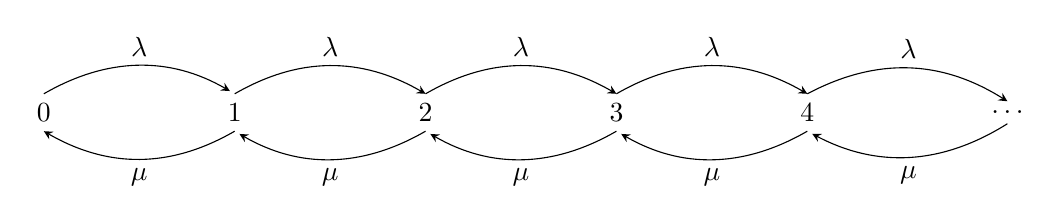
\begin{tikzpicture}
              \node (a) {0};
              \node[right=2cm of a] (b) {1};
              \node[right=2cm of b] (c) {2};
              \node[right=2cm of c] (d) {3};
              \node[right=2cm of d] (e) {4};
              \node[right=2cm of e] (f) {$\ldots$};
            
              %a>b
              \draw[-stealth,shorten >= 2pt] (a.north) to[bend left] node[midway,above] {$\lambda$} (b.north);
              \draw[-stealth] (b.north) to[bend left] node[midway,above] {$\lambda$} (c.north);
              \draw[-stealth] (c.north) to[bend left] node[midway,above] {$\lambda$} (d.north);
              \draw[-stealth] (d.north) to[bend left] node[midway,above] {$\lambda$} (e.north);
              \draw[-stealth] (e.north) to[bend left] node[midway,above] {$\lambda$} (f.north);
            
              %b>a
              \draw[-stealth] (b.south) to[bend left] node[midway,below] {$\mu$} (a.south);
              \draw[-stealth,shorten >= 2pt] (d.south) to[bend left] node[midway,below] {$\mu$} (c.south);
              \draw[-stealth,shorten >= 2pt] (e.south) to[bend left] node[midway,below] {$\mu$} (d.south);
              \draw[-stealth,shorten >= 2pt] (f.south) to[bend left] node[midway,below] {$\mu$} (e.south);
              \draw[-stealth,shorten >= 2pt] (c.south) to[bend left] node[midway,below] {$\mu$} (b.south);
            \end{tikzpicture}
$$
    \begin{itemize}
        \item Birth-death chain (Population Model)
        \item M/M/1 queue
        $$\includegraphics[height=4cm, width=13cm]{CTMC_4.jpeg}$$
        
    \end{itemize}
\end{itemize}
\end{enumerate}

\vspace{2\baselineskip}
{\bf Example}\\ 
Suppose the current state is 3. Then the rate of jumping out of the state 3 is $\lambda + \mu$. And
$$\begin{cases}
\text{P(move to 4)}=\frac{\lambda}{\lambda+\mu}\\
\text{P(move to 2)}=\frac{\mu}{\lambda+\mu}\\
\end{cases}$$

{\bf Construction of $X_t,$ given the rates $\{q(x,y)\}_{x\neq y}$}
$$\lambda_x = \sum\limits{y:y\neq x} q(x,y) = \text{total rate to jump out of state $x$}$$
If $\lambda_x = \infty$, the Markov chain leaves state $x$ immediately, so we can ignore such states \& assume each $\lambda_x<\infty$. $\lambda_x=0$ means that $x$ is absorbing.

\vspace{1\baselineskip}
If $0<\lambda_x<\infty,$ we define a transition probability
$$r(x,y) = \frac{q(x,y)}{\lambda_x}$$

\underline{Aside:} Suppose $W\sim \exp(1)$\\
Let $\oversim{W} = \tilde{W}{\lambda}$
$$P(\tilde{W}>t) = P(W>\lambda t) = e^{-\lambda t} \Rightarrow \tilde{W}\sim \exp(\lambda)$$

Ingredients of the construction:
\begin{enumerate}[label=(\roman*)]
    \item A discrete-time Markov chain $(Y_n)_{n\ge 0}$ with $Y_0 \sim \mu$.
    \item IID sequence $(\tau_k)_{k\ge 0}$ with $\tau_k\sim \exp(1)$.
\end{enumerate}

\begin{itemize}
    \item $T_0 = 0$
    \item $T_1 = t_1 = \frac{\tau_0}{\lambda_{Y_0}}$
    \item $X_t = Y_0$ for $0\le t < T_1$
    \item $t_2 = \frac{Y_1}{\lambda_{Y_1}} \qquad T_2 = T_1+t_2$
    \item $X_t =Y_1$ for $T_1\le t < T_2$
\end{itemize}

Suppose we have constructed up to $T_n= t_1+...+t_n$ such that $X_t=y_k$ for $T_k\le t < T_{k+1}$ for $k=0,...,n-1$. \\

Next step:
$$t_{n+1} = \frac{\tau_n}{\lambda_{Y_n}}\qquad T_{n+1} = T_n +t_{n+1}\qquad X_t=Y_n \text{ for } T_n\le t < T_{n+1}$$
$$\includegraphics[height=6.5cm, width=13cm]{CTMC_5.jpeg}$$


Compute transition probability $P_t = (p_t(x,y))_{x,y\in S}$ (4.2 on Durrett)\\

This construction does satisfy
$$\lim\limits_{h\to 0} \frac{P_h(x,y)}{h} = q(x,y)$$
Differential equation: for transition probabilities. 

Chapmnan-Kolmogorov equations:
$$p_{t+s}(x,y) = \sum\limits_{z} p_t(x,z)p_s(z,y)$$
Think of $h>0$ small small

\begin{align}
   p_{t+h} - p_t(x,y) &= \sum\limits_z P_h(x,z)p_t(z,y)-p_t(x,y) \nonumber \\
            &=\sum\limits_{z\neq x}p_h(x,z)p_t(z,y) + (p_h(x,x)-1)p_t(x,y) \nonumber \\
    \frac{p_{t+h} - p_t(x,y)}{h} & = \underbrace{\sum\limits_{z\neq x} \frac{p_h(x,z)}{h}p_t(z,y)}_{\xrightarrow{h\to 0}q(x,z)}
    +\underbrace{\frac{p_n(x,x)-1}{h}p_t(x,y)    }_{
    -\sum\limits_{z\neq x}\frac{p_h(x,z)}{h} \xrightarrow{h\to 0}
    -\sum\limits_{z\neq x}q(x,z) = =\lambda_x} \nonumber \\
    \frac{d}{dt}p_t(x,y) & = \sum\limits_{z\neq x} q(x,z)p_t(z,y)+(-\lambda_x)p_t(x,y) = \sum\limits_z Q_{x,z}p_t(z,y)\nonumber \\
    \frac{d}{dt}P_t &= QP_t \qquad P_0 = I \tag*{Kolmogorov's Backward Equation}
\end{align}

$$\frac{d}{dt} P_t = \left[\frac{d}{dt}p_t(x,y)\right]_{x,y\in S}$$
Similar argument leads to Kolmogorov's forward equation. 
$$P_t' = P_tQ$$

{\bf Examples}
$$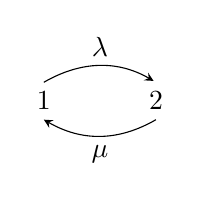
\begin{tikzpicture}
        \node (a) {1};
        \node[right=1cm of a] (b) {2};
        
        %a>b
        \draw[-stealth,shorten >= 1pt] (a.north) to[bend left] node[midway,above] {$\lambda$} (b.north);
        %b>a
        \draw[-stealth] (b.south) to[bend left] node[midway,below] {$\mu$} (a.south);
        \end{tikzpicture}\qquad
        Q=\begin{bmatrix}
        -\lambda&\lambda\\ \mu& -\mu
        \end{bmatrix}$$

\vspace{2\baselineskip}
Generator Matrix Q
$$Q_{x,z} = \begin{cases}q(x,z)&z\neq x\\-\lambda_x&z=x\end{cases}$$

2. $\mu/\mu/1$ queue
$$
            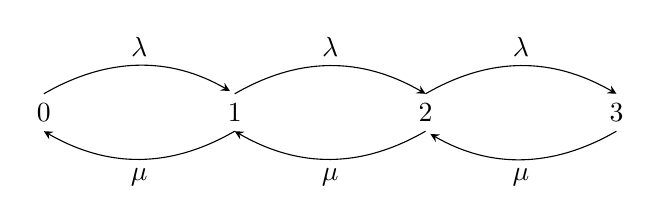
\begin{tikzpicture}
              \node (a) {0};
              \node[right=2cm of a] (b) {1};
              \node[right=2cm of b] (c) {2};
              \node[right=2cm of c] (d) {3};

            
              %a>b
              \draw[-stealth,shorten >= 2pt] (a.north) to[bend left] node[midway,above] {$\lambda$} (b.north);
              \draw[-stealth] (b.north) to[bend left] node[midway,above] {$\lambda$} (c.north);
              \draw[-stealth] (c.north) to[bend left] node[midway,above] {$\lambda$} (d.north);
              
            
              %b>a
              \draw[-stealth] (b.south) to[bend left] node[midway,below] {$\mu$} (a.south);
              \draw[-stealth] (c.south) to[bend left] node[midway,below] {$\mu$} (b.south);
              \draw[-stealth,shorten >= 2pt] (d.south) to[bend left] node[midway,below] {$\mu$} (c.south);
 
              
            \end{tikzpicture}
$$


$$
Q = \begin{matrix}
&{\bf 0}&{\bf 1}&{\bf 2}&{\bf 3}&{\bf 4}\\
{\bf 0}&-\lambda&\lambda&0&0&0&\ldots\\
{\bf 1}&\mu&-(\lambda+\mu)&\lambda&0&0&\ldots\\
{\bf 2}&0&\mu&-(\lambda+\mu)&\lambda&0&\ldots\\
{\bf 3}
\end{matrix}
$$


\vspace{2\baselineskip}
A probability mean $\mu$ on $S$ is an invariant distribution if $\pi=\piP_t\;\;\forall t\ge 0$.

\vspace{1.5\baselineskip}
{\bf Lemma 4.3} $\pi$ is invariant $\Leftrightarrow\; \pi Q = 0$ 

{\sl Proof} Assume $\pi$ is invariant\\

$\Rightarrow\; \pi = \pi P_t\;\;\forall t\ge 0$

\begin{align}
    0=\frac{d}{dt}(\pi P_t) &= \pi\frac{d}{dt}(P_t) = \pi P_t Q = \pi Q \nonumber \\
    \textit{Assume $\pi Q=0$\qquad}&\frac{d}{dt}(\pi P_t) = \pi\frac{d}{dt}(P_t)=\pi Q P_t = 0\cdot P_t = 0 \nonumber \\
    &\pi P_t = \pi P_0 = \pi \nonumber
\end{align}
So $\pi$ is invariant.

\newpage
Today
\begin{enumerate}
    \item Detailed Balance
    \item Queing Models
    \item Matrix Exponentials \& Solving Kolmogorov's Equations
    \item Blow-up
\end{enumerate}

\vspace{2\baselineskip}
1. Detailed Balance\\

Last time: $\pi$ is invariant if and only if $\pi Q=0$.\\

{\bf Definition} $\pi$ is a \underline{reversible distribution} (satisfies detailed balance) if
$$\pi(x)q(x,y) = \pi(y)q(y,x)\;\;\forall x\neq y$$

\vspace{1\baselineskip}
\underline{Fact:} If we start the Markov chain with a reversible distribution $\pi$, the time reversed process has the same distribution as the original process.

\vspace{1\baselineskip}
{\bf Theorem 4.5} Detailed balance $\Rightarrow \pi$ is invariant.

{\sl Proof.} \\
\begin{align}
(\pi Q)_y &= [\ldots\ldots ] 
\begin{bmatrix}
&&\vdots&&\\&&\vdots&&\\&&\vdots&&\\&&\vdots&&
\end{bmatrix} \nonumber \\
&=\sum\limits_x \pi(x)q(x,y) 
=\pi(y)q(y,y) + \sum\limits_{x\neq y} \pi(x)q(x,y) \nonumber \\
& = \pi(y)(-\lambda y) + \sum\limits_{x\neq y} \pi(y)q(y,x) 
=\pi(y)\left( = 0-\lambda_y + \underbrace{\sum\limits_xq(y,x)}_{\text{total rate out of y}} \right) \nonumber
\end{align}

{\bf Example}: M/M/1 queue
$$
            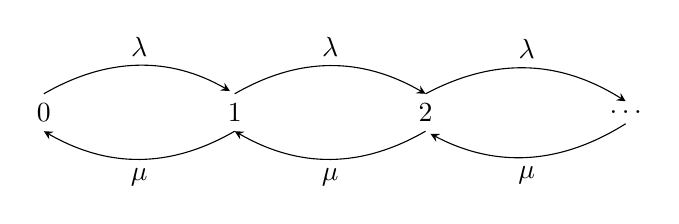
\begin{tikzpicture}
              \node (a) {0};
              \node[right=2cm of a] (b) {1};
              \node[right=2cm of b] (c) {2};
              \node[right=2cm of c] (d) {$\ldots$};

            
              %a>b
              \draw[-stealth,shorten >= 2pt] (a.north) to[bend left] node[midway,above] {$\lambda$} (b.north);
              \draw[-stealth] (b.north) to[bend left] node[midway,above] {$\lambda$} (c.north);
              \draw[-stealth] (c.north) to[bend left] node[midway,above] {$\lambda$} (d.north);
              
            
              %b>a
              \draw[-stealth] (b.south) to[bend left] node[midway,below] {$\mu$} (a.south);
              \draw[-stealth] (c.south) to[bend left] node[midway,below] {$\mu$} (b.south);
              \draw[-stealth,shorten >= 2pt] (d.south) to[bend left] node[midway,below] {$\mu$} (c.south);
 
              
            \end{tikzpicture}
$$

$$\begin{cases}
q(n,n+1)=\lambda &\text{for $n\ge 0$}\\
q(n,n-1)=\mu & \text{for $n\ge$1}
\end{cases}$$

Try to find a reversible distribution:
\begin{align}
    \pi_n q(n,n+1)&=\pi_{n+1}q(n+1,n)\nonumber \\
    &\Leftrightarrow \lambda\pi_n = \mu\pi_{n+1}\nonumber \\
    &\Leftrightarrow \pi_{n+1} = \frac{\lambda}{\mu}\pi_n \nonumber
\end{align}

So then
$$\pi_n=\frac{\lambda}{\mu}\pi_{n-1}=\left(\frac{\lambda}{\mu}\right)^2\pi_{n-2} = \ldots = \left(\frac{\lambda}{\mu}\right)^n\pi_0$$


\vspace{1\baselineskip}
\underline{continue:} To have a probability distribution, we want 
$$1=\sum\limits_{n=0}^\infty=\pi_n=\sum\limits_{n=0}^\infty\left(\frac{\lambda}{\mu}\right)^n\pi_9$$

If $\frac{\lambda}{\mu}<1$, we can solve for $\pi_0$:
\begin{align}
    1 &=\pi \sum\limits_{n=0}^\infty \left(\frac{\lambda}{\mu}\right)^n \nonumber \\
    &=\pi_0 \frac{1}{1-\frac{\lambda}{\mu}} \Rightarrow \pi_0 = 1-\frac{\lambda}{\mu} \nonumber
\end{align}

Answer: provided $\lambda<\mu$, where $\lambda$ is arrival rate and $\mu$ is service rate, we have a reversible distribution
$$\pi_n = \left(1-\frac{\lambda}{\mu}\right) \left(\frac{\lambda}{\mu}\right)^n \;\;\text{ for $n\ge 0$} \qquad\qquad \text{               (shifted geometric)}$$

Recall from HomeWork 3:
 $$
            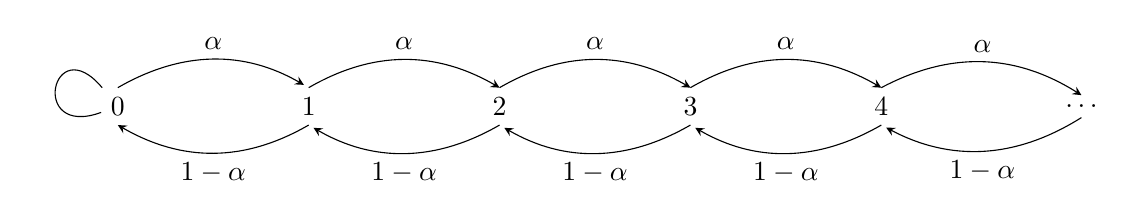
\begin{tikzpicture}
              \node (a) {0};
              \node[right=2cm of a] (b) {1};
              \node[right=2cm of b] (c) {2};
              \node[right=2cm of c] (d) {3};
              \node[right=2cm of d] (e) {4};
              \node[right=2cm of e] (f) {$\ldots$};
            
              \draw (a) to [out=130,in=200,looseness=8] (a);
              %a>b
              \draw[-stealth,shorten >= 2pt] (a.north) to[bend left] node[midway,above] {$\alpha$} (b.north);
              
              %b>c
              \draw[-stealth] (b.north) to[bend left] node[midway,above] {$\alpha$} (c.north);
              \draw[-stealth] (c.north) to[bend left] node[midway,above] {$\alpha$} (d.north);
              \draw[-stealth] (d.north) to[bend left] node[midway,above] {$\alpha$} (e.north);
              \draw[-stealth] (e.north) to[bend left] node[midway,above] {$\alpha$} (f.north);
            
              %b>a
              \draw[-stealth] (b.south) to[bend left] node[midway,below] {$1-\alpha$} (a.south);
              
              %c>b
              \draw[-stealth,shorten >= 2pt] (d.south) to[bend left] node[midway,below] {$1-\alpha$} (c.south);
              \draw[-stealth,shorten >= 2pt] (e.south) to[bend left] node[midway,below] {$1-\alpha$} (d.south);
              \draw[-stealth,shorten >= 2pt] (f.south) to[bend left] node[midway,below] {$1-\alpha$} (e.south);
              \draw[-stealth,shorten >= 2pt] (c.south) to[bend left] node[midway,below] {$1-\alpha$} (b.south);
            \end{tikzpicture}
            $$
            
This Markov chain has an invariant distribution if and only if $\alpha < \frac{1}{2}$.

\newpage
2. Queuing Models.
$$\includegraphics[height=8cm, width=13cm]{CTMC_6.jpeg}$$

\vspace{1\baselineskip}
Suppose $X_t=$ the number of customers in the system at time $t$, and let state space $S = \{0,1,2,...\}$. Then what is the rates?

\begin{align}
q(n,n+1) &= \lambda,\; n\ge 0\nonumber \\
q(n,n-1) &= \begin{cases} n\mu &1\le n<s \\ s\mu&n\ge s\end{cases}\nonumber \end{align} 

\vspace{1\baselineskip}
{\bf Fundamental fact:} If $W_1,...,W_n$ are independent random varialbes $W_i\sim \exp(\lambda_i),$ and $W=\min\limits_{i\le 1\le n}W_i$ then $W\sim \exp(\lambda_1+...+\lambda_n).$

\vspace{1\baselineskip}
{\bf M/M/S queue with balking}\\
Suppose an arriving customer who sees $n$ customers in the system, \underline{leaves} with probability $b_n$.\\

\underline{Rates:}
\begin{align}
    q(n,n+1)=a_n\lambda \text{ where $a_n=1-b_n$}\nonumber \\
    q(n,n-1) \text{   same as before} \nonumber
\end{align}


\newpage
{\bf M/M/$\infty$ queue}\\
Same rules as before except now the number of servers is unlimited so each arriving customers goes directly into service.
\begin{align}
    q(n,n+1)&=\lambda\nonumber \\
    q(n,n-1)&=n\mu \nonumber
\end{align}

{\bf Detailed Balance}\\
\begin{align}
    \pi(n)q(n,n+1)&=\pi(n+1)q(n+1,n) \nonumber \\
    \pi(n)\lambda &= \pi(n+1)\cdot (n+1)\mu \nonumber \\
    \Rightarrow \pi(n+1) &= \frac{\lambda/\mu}{n+1}\pi(n) = \frac{(\lambda/\mu)^2}{(n+1)n}\pi(n-1) \nonumber \\
    &=\ldots = \frac{(\lambda/\mu)^{n+1}}{(n+1)!}\pi_0^{e^{}/-\lambda/\mu} \nonumber
\end{align}

So $$\pi(n)=e^{-\lambda/\mu} \frac{(\lambda/\mu)^n}{n!} \sim \text{Poisson}\left(\frac{\lambda}{\mu}\right)$$

\vspace{2\baselineskip}
{\bf Scalar Version}
\begin{align}
    x'(t)&=qx(t) \nonumber \\
    x(0)&=1 \nonumber
\end{align}

Solution:
\begin{align}
    x(t)&=e^{tq}\nonumber \\
    e^x&=\sum\limits_{k=0}^\infty \frac{x^k}{k!}\nonumber
\end{align}

\begin{align}
    P_t' &= QP_t = P_t Q\nonumber \\
    P_0&=I\nonumber
\end{align}

Define a matrix exponential
$$e^{tQ} = \sum\limits_{k=0}^\infty \frac{t^kQ^k}{k!}$$

\vspace{1\baselineskip}
\underline{Fact:} this series converges for any finite matrix.

\vspace{2\baselineskip}
Let's see if $P_t=e^{tQ}$ solves.
\begin{align}
    \frac{d}{dt}e^{tQ} &= \frac{d}{dt} \sum\limits{k=0}^\infty \frac{t^kQ^k}{k!} \nonumber \\
    &=\sum\limits_{k=0}^\infty \frac{d}{dt} \left(\frac{t^kQ^k}{k!}\right)= \sum\limits_{k=0}^\infty\frac{kt^{k-1}Q^k}{k!}=\sum\limits_{k=0}^\infty \frac{t^{k-1}Q^k}{(k-1)!} \nonumber \\
    &=Q\sum\limits_{k=0}^\infty \frac{t^{k-1}Q^{k-1}}{(k-1)!} = Qe^{tQ} \tag{Or, similarly, =$e^{tQ}Q$}
\end{align}

We have shown here $P_t=e^{tQ}$ satisfies 
\begin{align}
    P_t' &= QP_t = P_tQ\nonumber \\
    e^{tQ} &= I + \sum\limits_{k=0}^\infty \frac{t^kQ^k}{k!} \tag{$Q^0=I$} \\
    t&=0: e^{0\cdot Q} = I \nonumber
\end{align}

In some literature, $e^{tQ}$ is used as an alternative to $P_t$.


\vspace{2\baselineskip}
{\bf Examples}
$$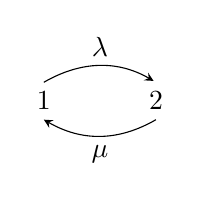
\begin{tikzpicture}
        \node (a) {1};
        \node[right=1cm of a] (b) {2};
        
        %a>b
        \draw[-stealth,shorten >= 1pt] (a.north) to[bend left] node[midway,above] {$\lambda$} (b.north);
        %b>a
        \draw[-stealth] (b.south) to[bend left] node[midway,below] {$\mu$} (a.south);
        \end{tikzpicture}\qquad
        Q=\begin{bmatrix}
        -\lambda&\lambda\\ \mu& -\mu
        \end{bmatrix}$$
        
Diagonalize $Q$: \\      
Idea: write $Q = B \wedge B^{-1}$ where $B$ is is eigen-vectors and $\wedge$ is diagonal matrix of eigenvalues.

\begin{align}
    Q^n & = B \wedge \underbrace{B^{-1}\cdot B}_I \wedge B^{-1}\cdot \ldots B \wedge B^{-1} = B \wedge B^{-1}\nonumber
\end{align}

$$\begin{matrix}
\text{Eigenvalues}&0&-(\lambda+\mu)\\
\text{Eigenvectors}&\binom{1}{1}&\binom{\lambda}{-\mu}
\end{matrix}\qquad
B=\begin{bmatrix}
1&\lambda \\1&-\mu
\end{bmatrix}\qquad$$

\begin{align}
B^{-1}&=\frac{1}{\lambda+\mu}\begin{bmatrix}
\mu&\lambda\\1&-1 
\end{bmatrix}
=B\underbrace{\left(\sum\limits_{n=0}^\infty \frac{t^n}{n!} 
\begin{bmatrix}
0&0\\0&-\mu-\lambda
\end{bmatrix}^n
\right)}_{\begin{bmatrix}
1&0\\0&e^{-t(\lambda+\mu)}
\end{bmatrix}}B^{-1} \nonumber \\
&=\begin{bmatrix}1&\lambda \\ 1 &-\mu \end{bmatrix}
\begin{bmatrix}1&0\\0&e^{-t(\lambda+\mu)}\end{bmatrix}
\frac{1}{\lambda+\mu}\begin{bmatrix}\mu&\lambda\\1&-1\end{bmatrix} \nonumber \\
&=\frac{1}{\lambda+\mu} \begin{bmatrix}1&\lambda e^{-t(\lambda+\mu)} \\ 1 &-\mu e^{-t(\lambda+\mu)} \end{bmatrix}
\begin{bmatrix}\mu&\lambda\\1&-1\end{bmatrix} \nonumber \\
&=\frac{1}{\lambda+\mu}\begin{bmatrix}
\mu+\lambda e^{-t(\lambda+\mu)}&\lambda - \lambda e^{-t(\lambda+\mu)} \nonumber \\
\mu-\mu e^{-t(\lambda+\mu)} & \lambda + \mu e^{-t(\lambda+\mu)}
\end{bmatrix} \nonumber \nonumber
\end{align}
$$
\lim\limits_{t\to\infty} P_t = 
\begin{bmatrix}
\frac{\mu}{\lambda+\mu}&\frac{\lambda}{\lambda+\mu} \\
\frac{\mu}{\lambda+\mu}&\frac{\lambda}{\lambda+\mu}\end{bmatrix}
=\begin{bmatrix}\pi\\ \pi\end{bmatrix}
$$
\end{document}